\documentclass[16pt, report]{article}
\usepackage[utf8]{inputenc}
\usepackage[a4paper, total={6in, 8in}]{geometry}
\usepackage{graphicx}
\graphicspath{{images/}}
\usepackage{amssymb}
\title{AI1110 Assignment 1}
\author{Hema Sri Cheekatla, CS21BTECH11013}
\begin{document}
\maketitle
ISCE 10 2018
\section*{Question 4a}
Solve the following inequation, write down the solution set and represent it on the real number line:

\[  -2 + 10x \leq 13x + 10 < 24 + 10x,  x\in \mathbb{Z} \]

\section*{Solution}
\[  -2 + 10x \leq 13x + 10 < 24 + 10x\]
There are two inequation in the above expression
let us consider each inequation one at a time and find out the set of integers that obey the each inequation\newline
finally the intersection of the two sets gives us the set of integers that obey the entire expression

\subsection*{First Inequality}
$\hspace{16pt}\hspace{16pt} -2+10x \leq 13x+10$

$\Rightarrow -2-10 \leq 13x-10x$

$\Rightarrow -12 \leq 3x$

$\Rightarrow -4 \leq x$

$\Rightarrow x \geq -4$

and $x\in \mathbb{Z}$

therefore $x =\{ -4, -3, -2, -1, 0, 1, 2,\dots\} \longrightarrow set1$

\subsection*{Second Inequality}
$\hspace{16pt}\hspace{16pt} 13x+10 < 24+10x$

$\Rightarrow 13x-10x < 24-10$

$\Rightarrow 3x < 14$

$\Rightarrow x < 14/3$

$\Rightarrow x < 4.6667$

and $x\in\mathbb{Z}$

therefore $x = \{ 4, 3, 2, 1, 0, -1, -2,\dots\} \longrightarrow set2$

Now the intersection of these two sets gives us the actual set of integers that obey the given expression

\begin{center}
\begin{tabular}{|c|}
\hline
\textbf{$set1 \cap set2 = \{ -4, -3, -2, -1, 0, 1, 2, 3, 4\}$} \\
\hline
\end{tabular}
\end{center}


here is the plot of corresponding points on the real number line
\begin{figure}[h]

    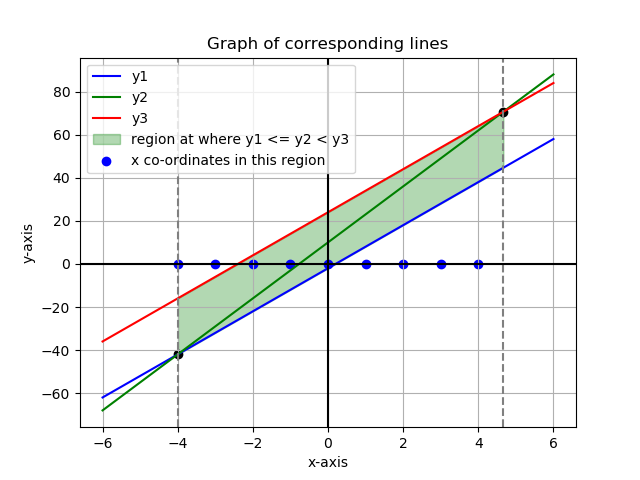
\includegraphics{Figure_1}
    \caption{set of points that obey given expression on real number line}
    \label{fig:mesh1}
\end{figure}
\end{document}
